\newpage
\thispagestyle{empty}
%\chpage
%\begin{adjustwidth*}{-2em}{-2em}


\noindent\begin{minipage}[t]{0.29\textwidth}
	\vspace{0pt}
    
\includegraphics[width=\textwidth]{images/biorad_color.pdf}
\end{minipage}
%\hspace{1cm}
\hfill
\begin{minipage}[t]{0.65\textwidth}
	\vspace{0pt}\raggedright
	\noindent\textbf{\Large{Система экспрессии и выделения рекомбинантных белков \mbox{Profinity eXact\textsuperscript{TM}}}}
\end{minipage}

\bigskip

\bigskip

\large{
\begin{minipage}[t]{0.45\textwidth}
	\vspace{0pt}
%\raggedright
\begin{enumerate}[noitemsep, topsep=0em, partopsep=1em, leftmargin=0em]
%\begin{itemize}
	%\renewcommand{\labelitemi}{\checkmark}
\item[\Checkmark] Новая надёжная альтернатива системам с His-тэгом
\item[\Checkmark] Быстрое выделение и отщепление тега на колонке в один шаг
\item[\Checkmark] Без свободной протеазы
\item[\Checkmark] Без загрязнения тэгом
\item[\Checkmark] Нативные или денатурирующие условия
\item[\Checkmark] Высокая чистота рекомбинантного белка
\item[\Checkmark] Регенерируемые многоразовые картриджи
%\end{itemize}
\end{enumerate}

\end{minipage}
%\hfill
\begin{minipage}[t]{0.35\textwidth}
	\vspace{5em}\raggedright
	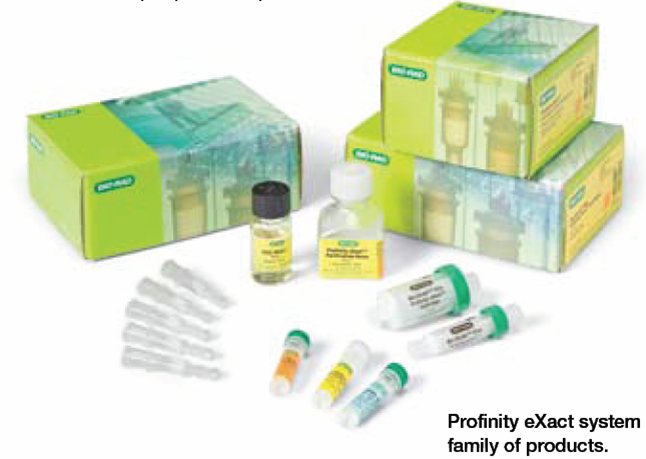
\includegraphics[width=1.3\textwidth]{images/exact1_color.png}
\end{minipage}

\begin{center}

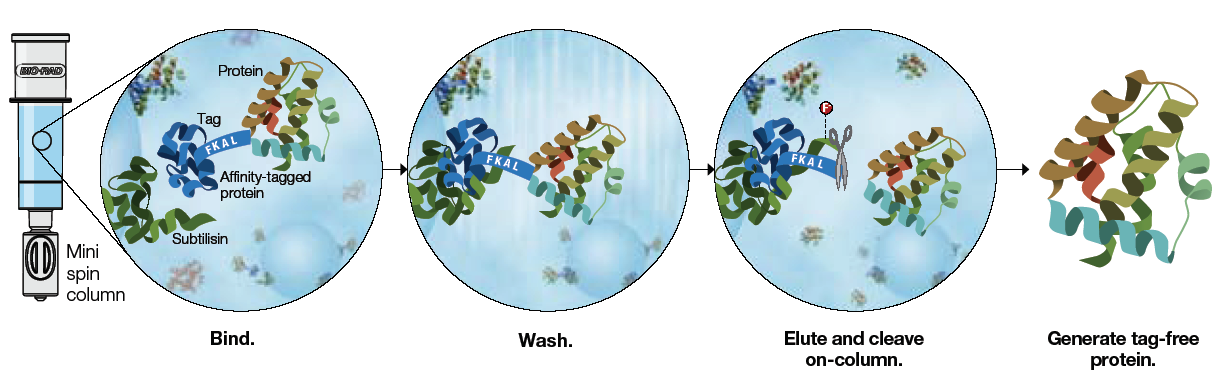
\includegraphics[width=0.9\textwidth]{images/exact2_color.png}

\noindent\textbf{Принцип работы системы Profinity eXact \textsuperscript{TM}}
\end{center}

\noindent\small{Тэгом является про-домен субтилизинина. Протеаза (субтилизин) иммобилизована на колонке. При загрузке колонки протеаза эффективно связывает про-домен. Промывка специальным буфером активирует протеазную активность. Тэг при этом остаётся надёжно связанным с протеазой и не вымывается с колонки. Чистый белок без тега и протеазы выходит в элюате. 

\begin{center}

02160, Киев, проспект Воссоединения 7а,  оф. 315 Тел. (044) 599-31-23,

Факс (044) 559-46-13 

e-mail: \email{office@bio-rad.com.ua}

\end{center}
}
%\end{adjustwidth*}

%\newpage
%\chback
